\documentclass[border=10pt]{standalone}
\usepackage{pgfplots}
\pgfplotsset{compat=1.18,trig format plots=rad}
\begin{document}
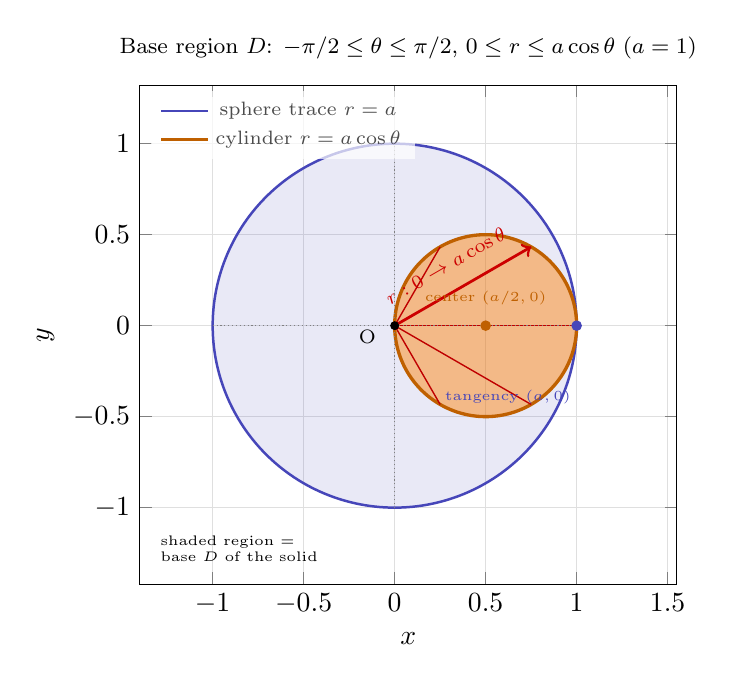
\begin{tikzpicture}
\begin{axis}[
  width=8.4cm,height=8.4cm,
  xmin=-1.40,xmax=1.55,ymin=-1.42,ymax=1.32,
  axis equal image,
  xlabel={$x$},ylabel={$y$},
  grid=major,grid style={gray!25},
  samples=240,
  legend style={draw=none,font=\scriptsize,at={(0.02,0.99)},anchor=north west,fill=white,fill opacity=.7},
  title={\footnotesize Base region $D$: $-\pi/2\le\theta\le\pi/2$, $0\le r\le a\cos\theta$ ($a=1$)}]

  \addplot+[fill=blue!45!gray,fill opacity=.12,draw=blue!45!gray,line width=0.9pt,
            domain=0:2*pi,mark=none] ({cos(x)},{sin(x)}) -- cycle;
  \addplot+[fill=orange,fill opacity=.45,draw=orange!75!black,line width=1.2pt,
            domain=-pi/2:pi/2,mark=none] ({cos(x)^2},{cos(x)*sin(x)}) -- cycle;

  \draw[red!75!black,line width=0.5pt] (axis cs:0,0) -- (axis cs:0.25,-0.433);
  \draw[red!75!black,line width=0.5pt] (axis cs:0,0) -- (axis cs:0.75,-0.433);
  \draw[red!75!black,line width=0.5pt] (axis cs:0,0) -- (axis cs:1,0);
  \draw[red!75!black,line width=0.5pt] (axis cs:0,0) -- (axis cs:0.75,0.433);
  \draw[red!75!black,line width=0.5pt] (axis cs:0,0) -- (axis cs:0.25,0.433);
  \draw[->,red!80!black,line width=1pt] (axis cs:0,0) -- (axis cs:0.75,0.433);
  \node[red!80!black,font=\scriptsize,rotate=30] at (axis cs:0.28,0.33) {$r:0 \to a\cos\theta$};

  \draw[gray,densely dotted,line width=0.4pt] (axis cs:-1,0) -- (axis cs:1,0);
  \draw[gray,densely dotted,line width=0.4pt] (axis cs:0,-1) -- (axis cs:0,1);

  \filldraw[orange!75!black] (axis cs:0.5,0) circle (1.7pt);
  \node[orange!75!black,font=\tiny,anchor=south] at (axis cs:0.5,0.06) {center $(a/2,0)$};
  \filldraw[blue!45!gray] (axis cs:1,0) circle (1.7pt);
  \node[blue!45!gray,font=\tiny,anchor=north east] at (axis cs:1.02,-0.30) {tangency $(a,0)$};
  \filldraw[black] (axis cs:0,0) circle (1.4pt);
  \node[font=\scriptsize,anchor=east] at (axis cs:-0.05,-0.06) {O};

  \node[font=\tiny,anchor=north west,text width=2.2cm,align=left] at (axis cs:-1.34,-1.10)
     {shaded region $=$ base $D$ of the solid};

  \addlegendentry{sphere trace $r=a$}
  \addlegendentry{cylinder $r=a\cos\theta$}
\end{axis}
\end{tikzpicture}
\end{document}
